% ---------------------------------------------------------------------------
% Compact narrative draft of the main text (Sections 1-6).
% Companion: theory_appendix_main_results.tex holds every statement in full,
% in derivation order.  Here propositions are stated only where they carry the
% story; everything else is a pointer.
%
% Figure plan (3 figures):
%   Fig 1  neuronal results (top row) + linear recapitulation (bottom row)
%   Fig 2  pixel ridge: landscape + CV path
%   Fig 3  feature ridge: dependency graph + null rotation + biological validation
%   wrapfig  iso-error geometry + ridge path (Sec 3)
% ---------------------------------------------------------------------------

\begin{abstract}
Models that predict visual-neuron responses similarly well on held-out images can differ sharply in the stimuli they generate and in their ability to control those neurons, and control success tracks the structure of a model's input gradient more closely than its predictive accuracy. We study this prediction--control dissociation in a linear teacher--student model. Ordinary generalization evaluates a fitted predictor on the natural-image distribution; feature accentuation evaluates it on a distribution generated along its own fitted direction. This change of distribution gives control error, $R^2$, and response slope a different dependence on estimation error than test loss: prediction weights weight error by the data covariance, control counts it in Euclidean geometry. Using deterministic equivalents for ridge regression we show that prediction-optimal and control-optimal regularization obey different spectral conditions, so cross-validation can leave large control error under noisy, anisotropic data. Extending the analysis to fixed linear feature maps, prediction depends only on the feature covariance and its alignment with the teacher, whereas control additionally depends on the map's Euclidean input-gradient geometry: control is most fragile when the feature directions that survive regularization backpropagate into low-variance, high-spatial-frequency image directions. The separation is exact: a gauge group of feature-map transformations, rotations in whitened input coordinates that fix the teacher, leaves generalization and its cross-validated optimum invariant while moving control from calibrated to arbitrarily poor. The resulting gradient-geometry factor extends to nonlinear networks as a diagnostic and recovers model-to-model variation in biological control that held-out accuracy does not.
\end{abstract}

\section{Introduction}
A predictive model of a neural population is, in principle, also a controller: if $f(\x)$ predicts the response of a neuron to an image $\x$, one can synthesize images that drive $f$ to a target level and present them to the neuron. Model-based control of visual neurons has recently been carried out at scale with deep-network encoding models and gradient-based stimulus synthesis \citepPW. The result is puzzling. Encoding models that are nearly indistinguishable on held-out natural images generate visibly different stimuli and differ several-fold in how well those stimuli modulate the neuron; models that fail to control can still recognize the successful stimuli of other models; and the best predictor of control success is not accuracy but the spectral structure of the model's input gradient.

We argue that none of this requires nonlinearity, depth or biology. It arises already for linear regression, from a single fact: \emph{control evaluates a model on a distribution the model itself generates}. Held-out prediction measures weight error in the metric of the data covariance $\Sigma$, which suppresses low-variance directions; accentuation moves along the fitted weight itself and therefore measures the same error in Euclidean geometry, where nothing is suppressed. For natural images, whose covariance spectrum decays over many orders of magnitude, this is the difference between not seeing an error and being dominated by it.

Our contributions are:
(i) a formulation of generalization, self-accentuation and peer review as evaluations of one predictor under three input distributions, with their equal-error sets (ellipsoid, sphere, hyperplane) exposing the dissociation geometrically (Sec.~\ref{sec:setup});
(ii) deterministic equivalents for pixel-space ridge regression showing that prediction-optimal and control-optimal penalties satisfy different spectral conditions, so cross-validation leaves a computable residual control error (Sec.~\ref{sec:pixel});
(iii) for regression on a fixed linear feature map, a separation of the summary statistics that determine prediction from those that determine control, and a gauge family of feature maps with identical generalization but arbitrarily different control (Sec.~\ref{sec:feature});
(iv) a response-independent gradient-geometry factor $T_F$ that identifies fragile feature maps, extends to nonlinear networks as a diagnostic, and recovers model ordering in the neuronal control data.
All statements are proved in the appendix, which also restates every result in derivation order (App.~\ref{sec:app-main-results}); numerical validation against Monte Carlo and natural-image regression accompanies each section.

\paragraph{Related work.}
High-dimensional ridge regression under anisotropic covariance is classical \citep{dobriban2018high,hastie2022surprises}, and deterministic equivalents for its risk are standard \citep{bai2010spectral,couillet2011random}; we use this toolkit but change the evaluation distribution from the training law to a model-generated path. Optimizing inputs against a fitted model is the setting of feature visualization and accentuation \citep{olah2017feature,hamblin2024feature}, adversarial examples and performative prediction; our contribution is a solvable model in which the resulting distribution shift is computed rather than assumed. Model-based closed-loop neuroscience \citepPW\ supplies the phenomena.

\section{Prediction and control dissociate in neurons and in linear regression}
\label{sec:phenomena}

\begin{figure}[t]
    \centering
    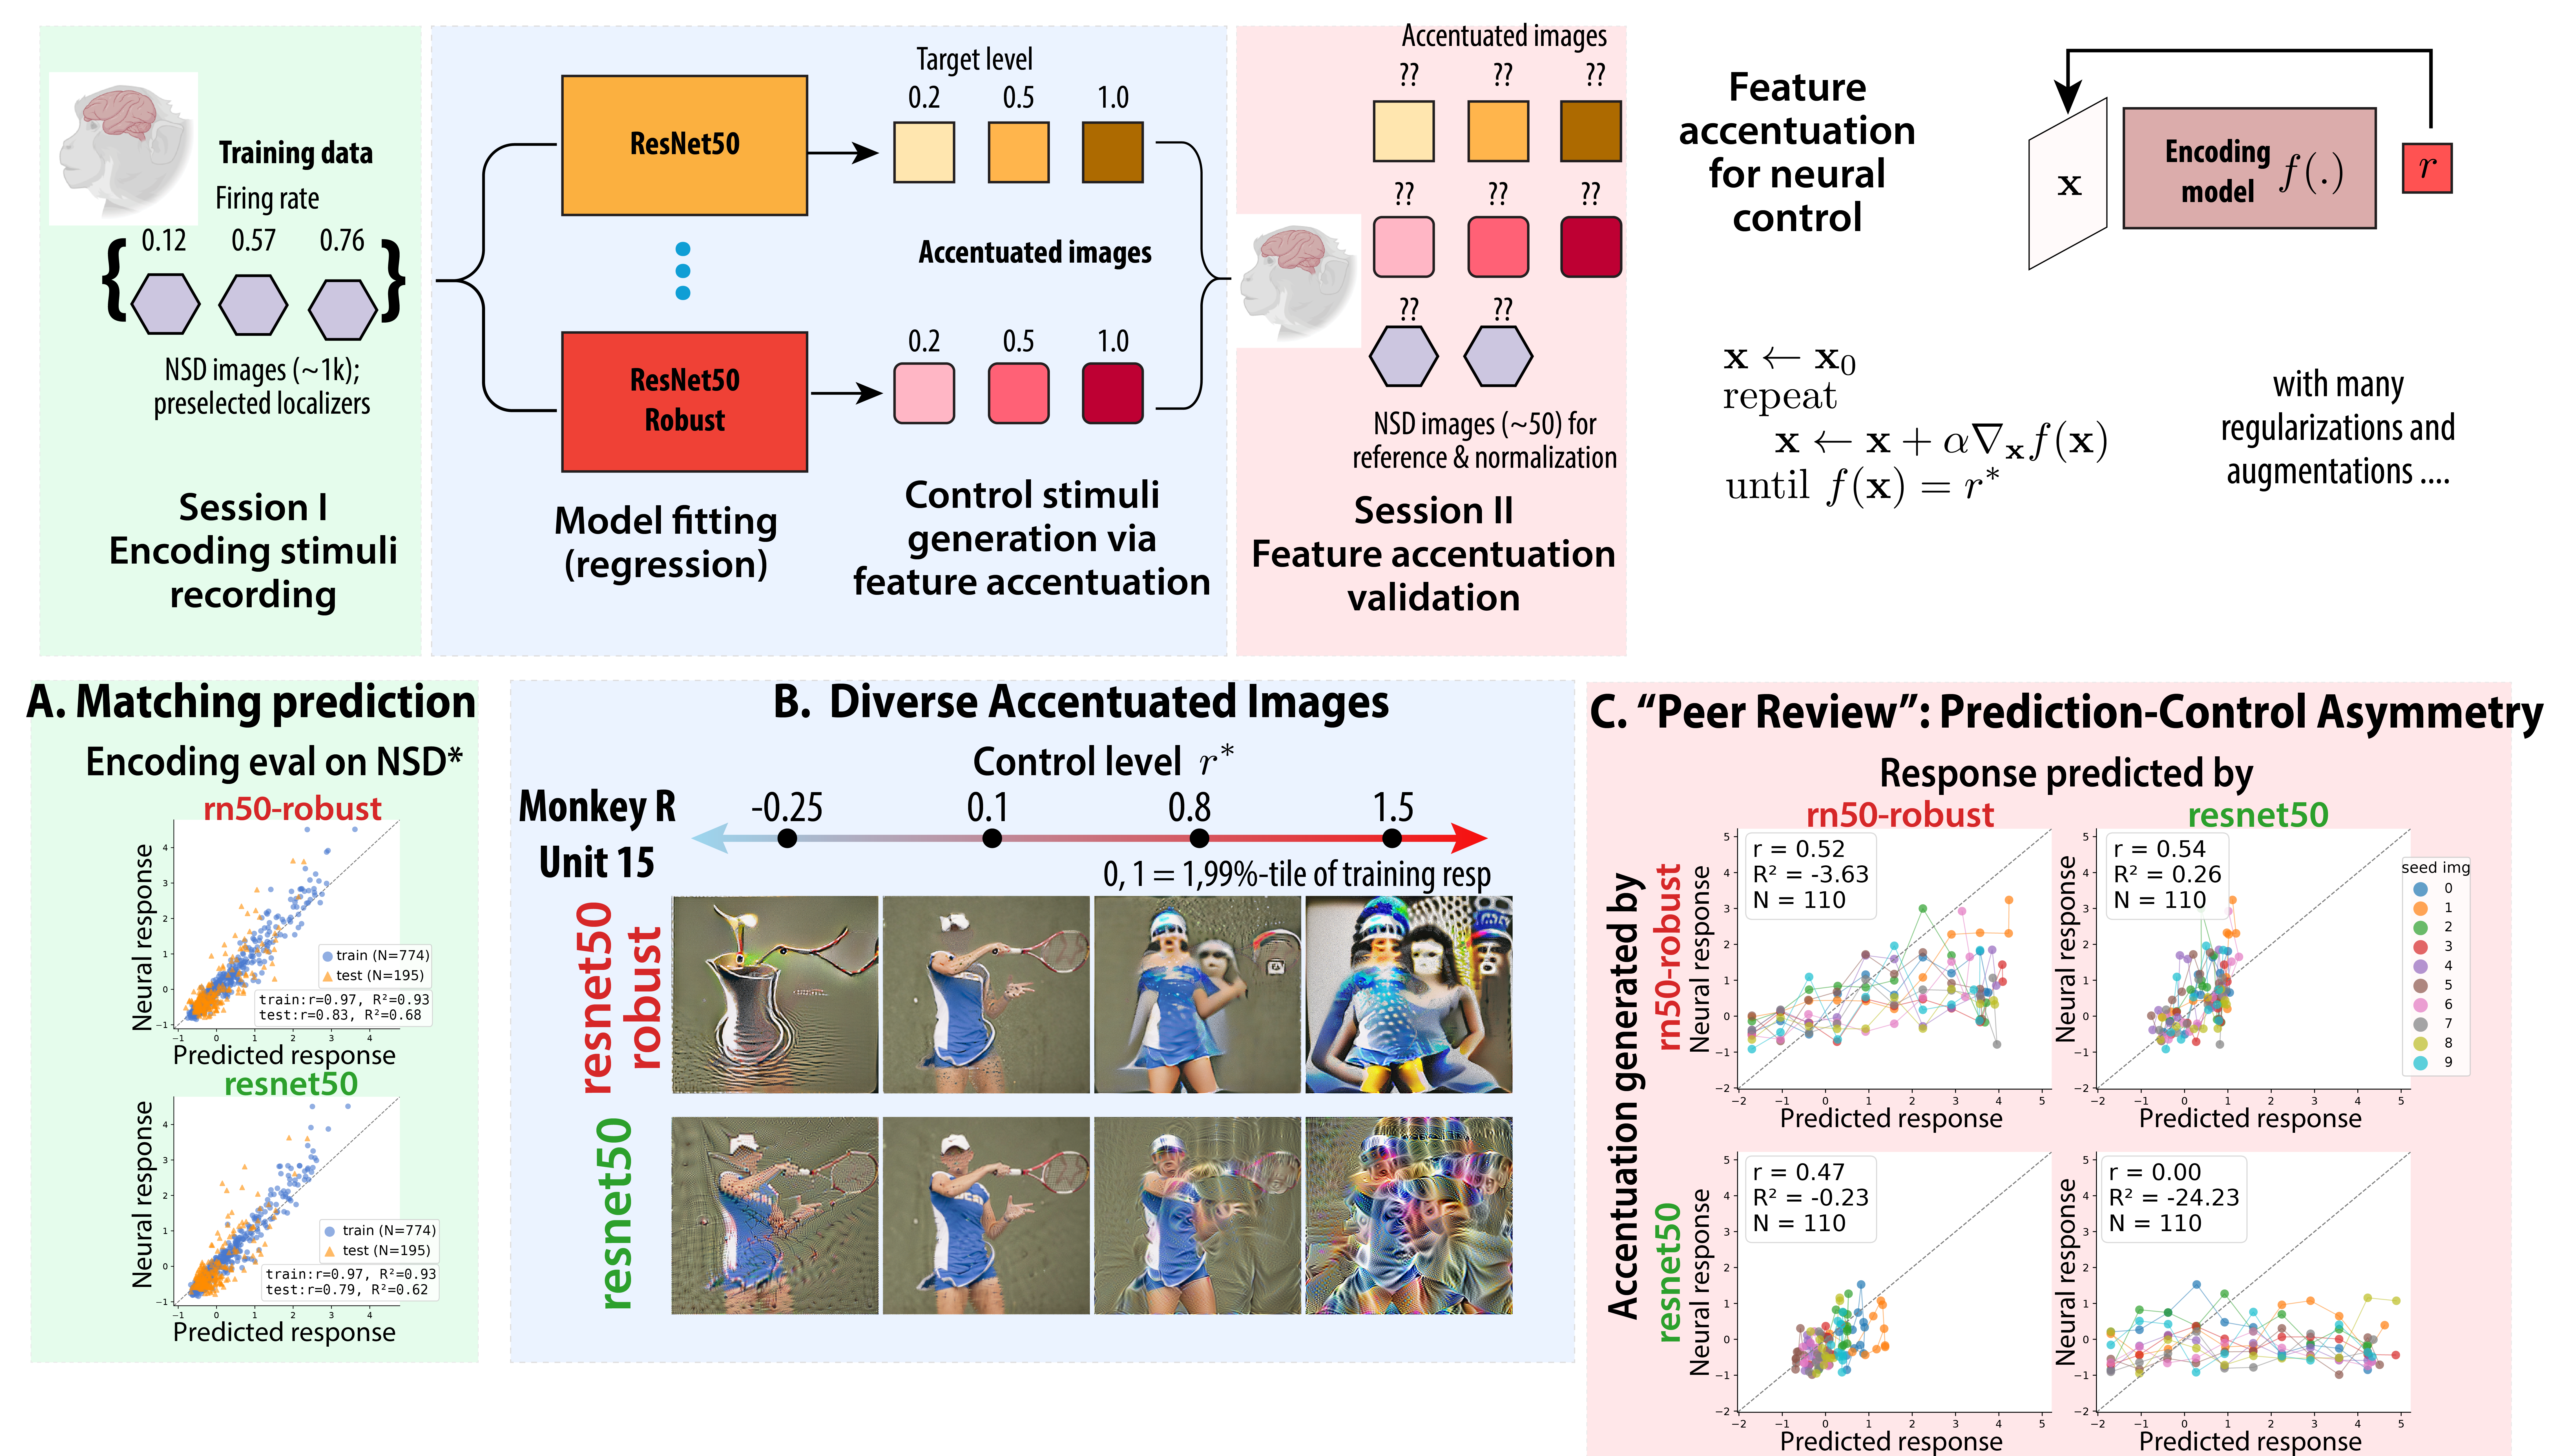
\includegraphics[width=\linewidth,height=0.27\textheight,keepaspectratio]{figures/Figure_NeuroCtrl_results.png}\\[2pt]
    \includegraphics[width=\linewidth,height=0.27\textheight,keepaspectratio]{figures/Figure_LinearToyModel.png}
    \caption{\textbf{The same three phenomena in neurons (top) and in a linear teacher--student model (bottom).}
    Top: closed-loop experiment of \citetPW. Encoding models are fit to responses to natural images, generate accentuated images for graded target responses, and are tested in a second session.
    \textbf{A}~Two models predict held-out natural-image responses equally well.
    \textbf{B}~Their accentuations from the same seed differ visibly, and only one modulates the neuron.
    \textbf{C}~Peer review: each model evaluated on the other's images. The weak controller tracks the strong controller's images but its own images barely modulate the neuron.
    Bottom: two linear students of a linear teacher (a disk-shaped weight on van~Hateren images), differing only along low-variance image directions, reproduce A--C exactly. Geometry inset: prediction sees weight error through the covariance ellipse; the accentuation path exposes the hidden Euclidean difference.}
    \label{fig:phenomena}
\end{figure}

Figure~\ref{fig:phenomena} (top) summarizes the closed-loop experiments of \citetPW: responses of visual cortical sites (V2--IT, 25 sites in 5 macaques) to $\sim$1000 natural images were recorded; ten deep-network encoding models were fit by ridge regression on network features with penalty and layer chosen by cross-validation; each model then synthesized, by gradient-based \emph{feature accentuation} \citep{hamblin2024feature}, images that drive its own prediction to eleven target levels from ten seed images; and the images were presented to the same sites. Three observations motivate this paper.

\paragraph{Similar prediction, divergent control.}
The trained models were tightly matched on held-out natural images, yet the slope and correlation between predicted and measured responses to their own accentuated images varied widely across models, with far larger spread than on natural images. Many models reached their requested \emph{predicted} response by adding texture and high-spatial-frequency structure that left the neuron largely unmoved.

\paragraph{Recognition without generation.}
Presenting model A's images to model B (``peer review'', Fig.~\ref{fig:phenomena}C) shows an asymmetry: a model whose own images fail to modulate the neuron still predicts the neuronal responses to a successful model's images with good correlation and better calibration than the generator itself. Models can recognize good control stimuli that they cannot produce.

\paragraph{Control tracks input-gradient structure.}
Across the 250 site--model pairs, control success is predicted by the spectral profile of the model's input gradient $\nabla_\x f$: models whose gradients concentrate power at low spatial frequencies, like natural images, control better. The two adversarially trained models are the strongest controllers, but the association persists without them.

The bottom row of Fig.~\ref{fig:phenomena} shows that a linear model reproduces all three observations once its weight error lies along low-variance directions of the image covariance. The remainder of the paper explains why finite-sample regression on noisy responses puts it there, why cross-validation does not remove it, and how the feature map decides how much of it reaches the pixel gradient.

\section{Three evaluations of one predictor}
\label{sec:setup}

\paragraph{Teacher and student.}
Inputs $\x\in\R^d$ are drawn from $\mathcal N(0,\Sigma)$ with $\Sigma=\sum_ks_k\uvec_k\uvec_k^\top$. A linear teacher with weight $\bstar=\sum_kb_k\uvec_k$ produces noisy responses $y=\x^\top\bstar+\sigma\epsilon$, and $S:={\bstar}^\top\Sigma\bstar$ is the natural response variance. The student is $f(\x)=\x^\top\bhat$, fitted from $n$ pairs $(X,\mathbf y)$; for feature-space students (Sec.~\ref{sec:feature}) $\bhat$ is the effective pixel weight $F^\top\hat w$, which is also the gradient $\nabla_\x f$.

\paragraph{Three distributions.}
Generalization evaluates $f$ on fresh natural inputs, $\x\sim\mathcal N(0,\Sigma)$. Accentuation evaluates $f$ on inputs it generates itself: gradient ascent from a seed $\x_0$ moves along $\nabla_\x f=\bhat$, so the idealized path is $\x=\x_0+\alpha\bhat$ with $\alpha$ set by the target level.\footnote{Deep-network accentuation adds preconditioning, augmentation and image priors \citep{hamblin2024feature}; App.~\ref{sec:app-evaluation-distributions} treats nonzero and multiple seeds.} In the main text $\x_0=0$ and the target range is variance-matched, $\Var[\alpha]({\bhat}^\top\bhat)^2=S$, so the student \emph{predicts} the natural response range along its path. Peer review evaluates $f$ on the path $\x_0+\alpha\bprime$ generated by another student $\bprime$. Writing $\Delta=\bhat-\bstar$ and applying the standard formulas for MSE, $R^2$ and the slope of true-on-predicted response to each distribution (App.~\ref{lem:mr-metrics}) gives Table~\ref{tab:evaluation-metrics}.

\begin{table}[t]
\centering\small
\begin{tabular}{@{}llccc@{}}
\toprule
Evaluation & Input covariance & MSE & $R^2$ & Slope \\
\midrule
Generalization & $\Sigma$ & $\Delta^\top\Sigma\Delta$ & $1-\Delta^\top\Sigma\Delta/S$ & ${\bhat}^\top\Sigma\bstar/{\bhat}^\top\Sigma\bhat$ \\
Accentuation & $\Var[\alpha]\,\bhat{\bhat}^\top$ & $S\,(1-N/D)^2$ & $1-(D/N-1)^2$ & $N/D$ \\
Peer review & $\Var[\alpha]\,\bprime{\bprime}^\top$ & $S\,({\bprime}^\top\Delta)^2/({\bprime}^\top\bprime)^2$ & $1-\big(\frac{{\bprime}^\top\bhat}{{\bprime}^\top\bstar}-1\big)^2$ & ${\bprime}^\top\bstar/{\bprime}^\top\bhat$ \\
\bottomrule
\end{tabular}
\caption{One fitted weight, three evaluation distributions. $N:={\bhat}^\top\bstar$, $D:={\bhat}^\top\bhat$. Pearson correlation is degenerate on a noiseless rank-one path and is omitted.}
\label{tab:evaluation-metrics}
\end{table}

\paragraph{Prediction is covariance-weighted, control is Euclidean.}
Generalization error is $\Delta^\top\Sigma\Delta$: a weight error along $\uvec_k$ costs $s_k$ times its squared length, so errors in low-variance directions are nearly invisible. Every accentuation metric, by contrast, is a function of the single scalar
\begin{equation}
z_{acc}:=\frac DN-1=\frac{{\bhat}^\top(\bhat-\bstar)}{{\bhat}^\top\bstar},
\qquad
\frac{E_{acc}}{S}=\Big(\frac{z}{1+z}\Big)^2,\quad R^2_{acc}=1-z^2,\quad \mathrm{slope}_{acc}=\frac{1}{1+z},
\label{eq:acc_metric_ND_depen}
\end{equation}
which weights $\Delta$ by $\bhat$ itself, with no covariance in sight. Geometrically (App.~\ref{prop:mr-iso-geometry}), the equal-$E_{gen}$ sets are ellipsoids around $\bstar$ elongated along low-variance axes, whereas the equal-$z_{acc}$ sets are Euclidean spheres with diameter from $0$ to $(1+z)\bstar$, and the equal-peer-error sets are hyperplanes normal to $\bprime$. A student can sit deep inside the prediction ellipsoid, far from the control sphere, and still lie on the peer hyperplane of a good generator: this is exactly the configuration of Fig.~\ref{fig:phenomena} (bottom), and it can be made arbitrarily extreme by adding weight along a direction with $s_k\to0$ (App.~\ref{ex:mr-dissociation}).

The remaining question is therefore not whether the dissociation is possible but when \emph{learning} produces it. Three ingredients are in play: finite-sample regression on noisy responses, the choice of regularization, and the feature map through which the gradient reaches the pixels. We take them in turn.

\section{Pixel-space ridge: noise, spectrum and the choice of regularization}
\label{sec:pixel}

Ridge regression in pixel space, $\bhat=\arg\min_\beta\frac1n\|X\beta-\mathbf y\|^2+\lambda\|\beta\|^2$, yields
\begin{equation}
\bhat=\underbrace{(\hat\Sigma+\lambda I)^{-1}\hat\Sigma\bstar}_{\text{shrunken signal}}
+\underbrace{\sigma(\hat\Sigma+\lambda I)^{-1}\tfrac1nX^\top\eta}_{\text{noise}},
\qquad \hat\Sigma=X^\top X/n .
\label{eq:ridge}
\end{equation}
Since ridge penalizes weight in low-variance directions, one might expect it to remove the hidden Euclidean error. We ask whether the error survives, and whether the cross-validated penalty removes it.

\begin{wrapfigure}{r}{0.5\linewidth}
    \vspace{-8pt}
    \centering
    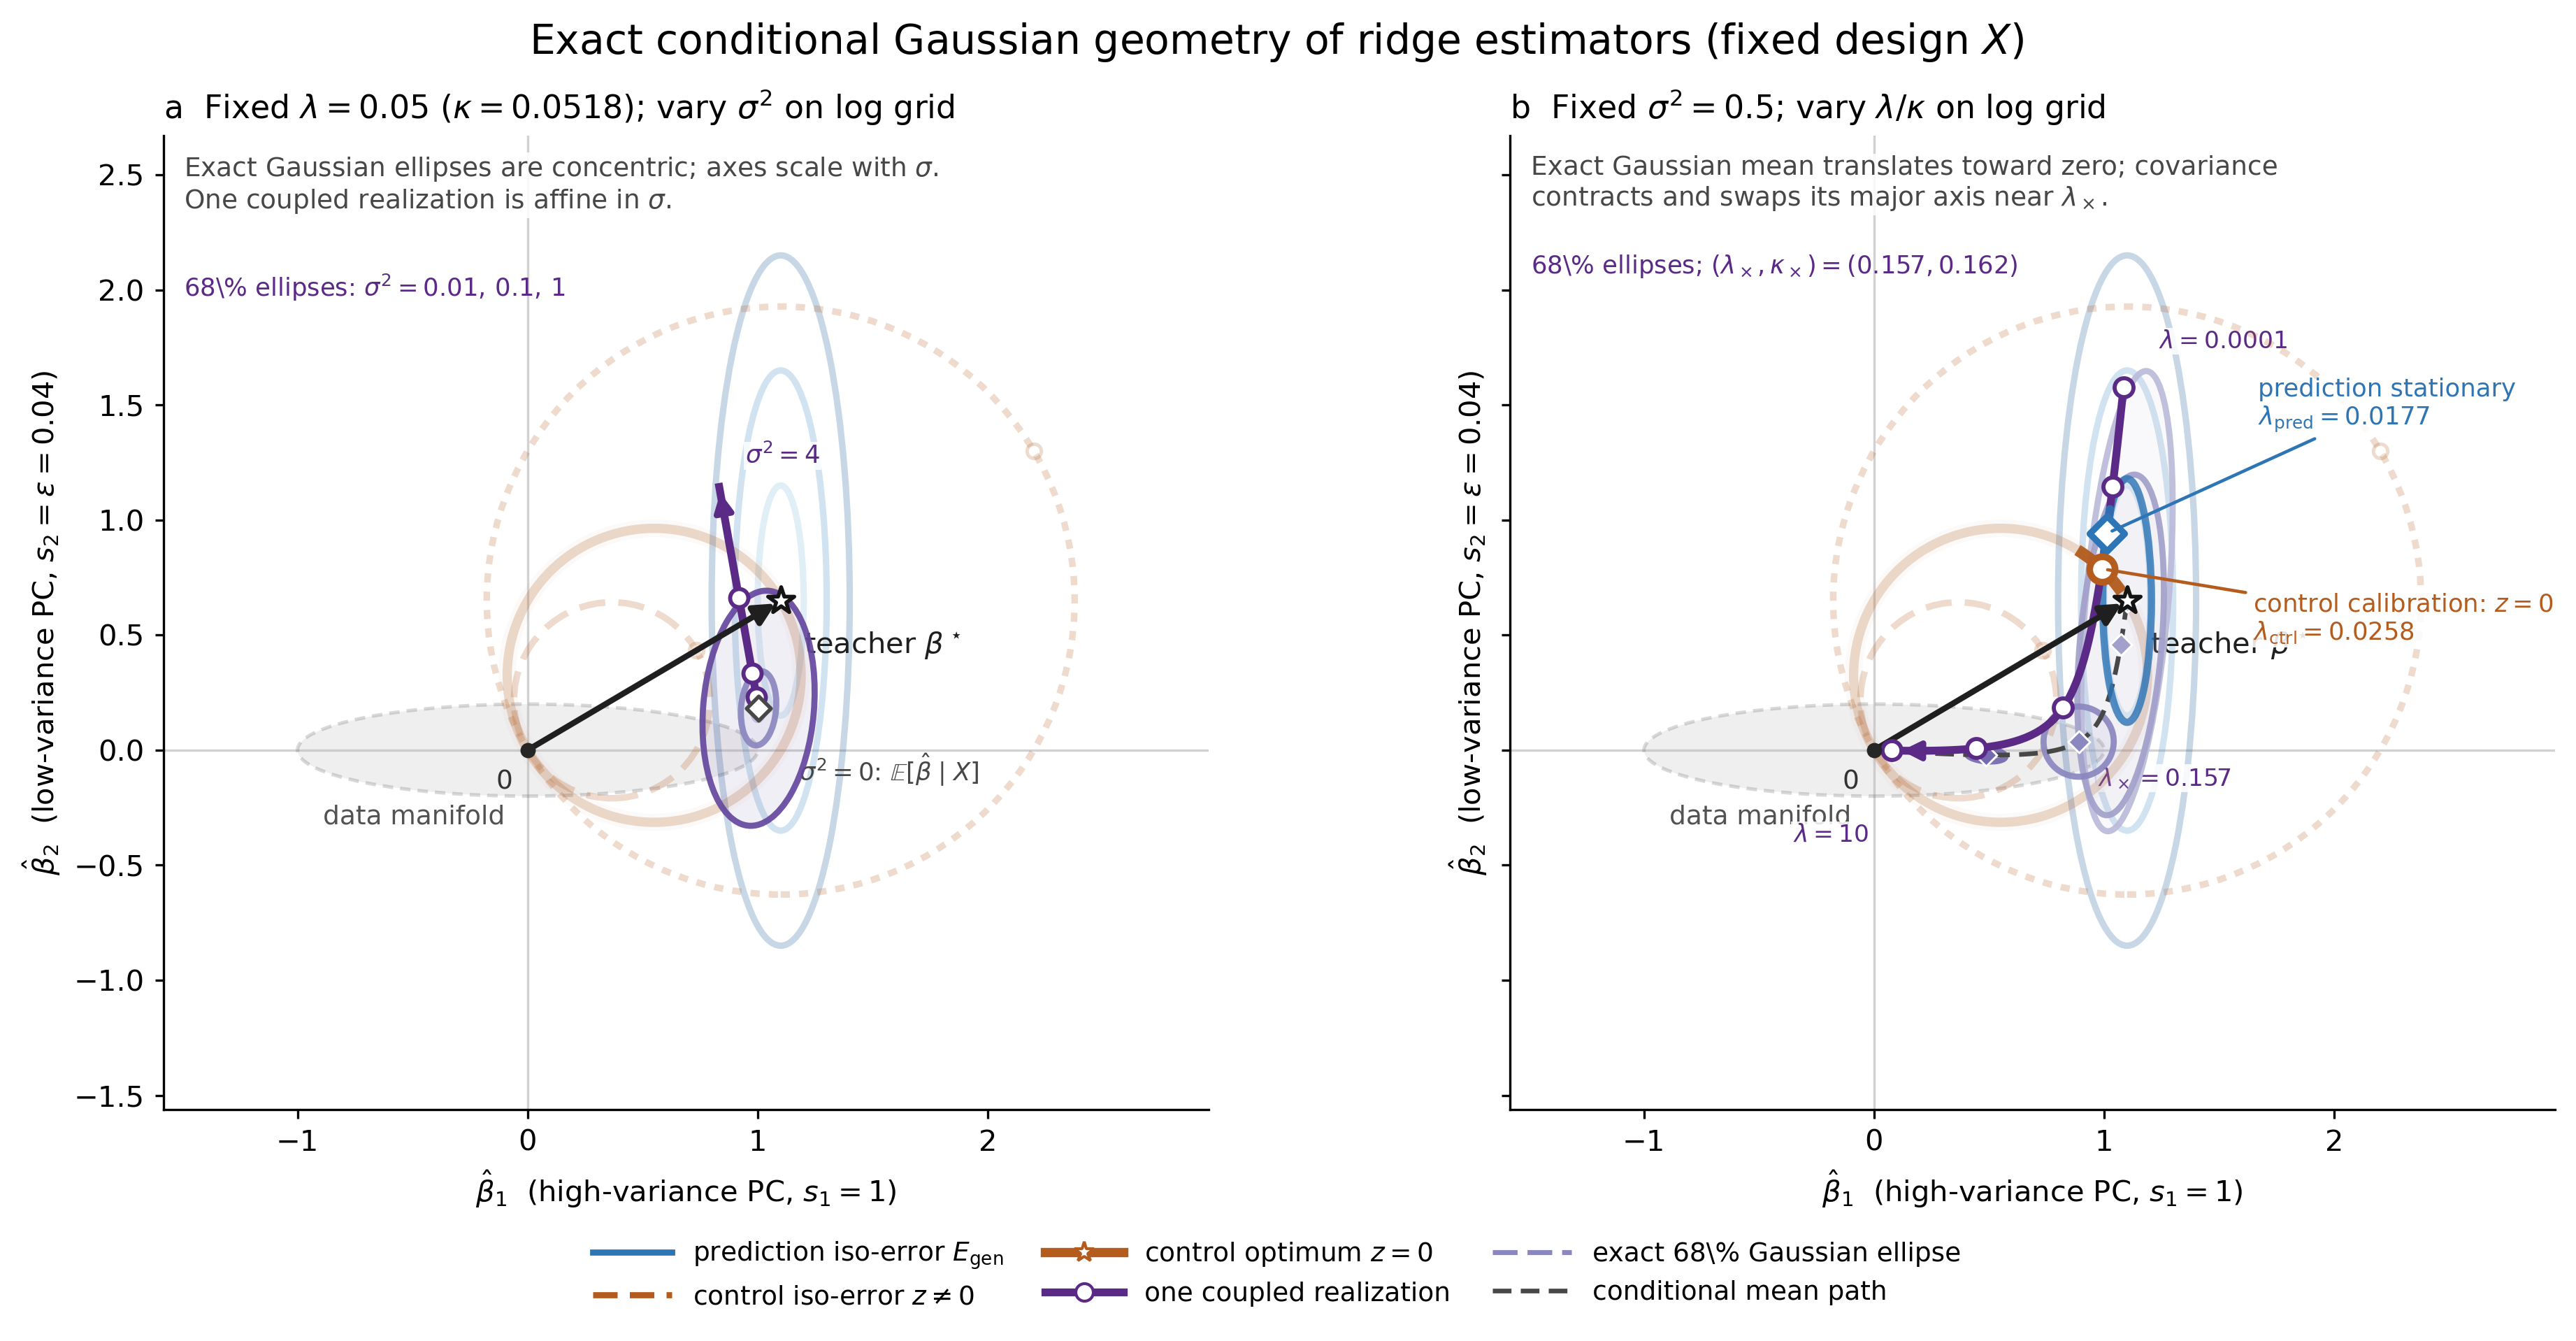
\includegraphics[width=\linewidth]{figures/draft_ridge_paths_iso_error_geometry.png}
    \caption{\textbf{Equal-error sets and the ridge path} in the plane of a high- and a low-variance PC. Prediction levels are ellipsoids around $\bstar$ (blue), control calibration is the sphere through $0$ and $\bstar$ (orange). The fitted weight is scattered around the ridge path (purple) with a spread elongated along the low-variance axis. Cross-validation picks the tangency of the path with an ellipsoid; control calibration is its crossing with the sphere. (Placeholder from the validation repository; to be polished.)}
    \label{fig:geometry}
    \vspace{-6pt}
\end{wrapfigure}
\paragraph{The ridge path through the two landscapes.}
The question has a geometric reading (Fig.~\ref{fig:geometry}). For a given training set, Eq.~\ref{eq:ridge} traces a path $\bhat(\lambda)$ in weight space from the least-squares or minimum-norm solution at $\lambda\to0$ to the origin at $\lambda\to\infty$. Response noise and the random design scatter the fitted weight in a cloud around this path, and the cloud is elongated along the low-variance directions of $\Sigma$, because those are the directions the data constrain least. Cross-validation selects the point of the path that is tangent to the smallest reachable prediction ellipsoid, whereas control calibration asks where the path crosses the sphere $D=N$; the two coincide only if the noise cloud has not pushed the path off the sphere in the directions the ellipsoid does not see. The deterministic equivalents below compute where the center of this cloud sits, how much Euclidean spread it carries, and hence the distance between the two points.


\paragraph{Toolkit.}
We use deterministic equivalents (DEs) in the proportional limit $d/n\to\gamma$ \citep{dobriban2018high,hastie2022surprises}. Finite-sample randomness enters through the effective penalty $\kappa(\lambda)$, the positive root of $\kappa-\lambda=\frac{\kappa}{n}\operatorname{Tr}[\Sigma(\Sigma+\kappa I)^{-1}]$, and the results are expressed through the teacher-weighted and unweighted spectral sums
\begin{equation}
B_{p,q}(\kappa)=\sum_k\frac{s_k^p}{(s_k+\kappa)^q}b_k^2,\qquad
\mathrm{df}_{p,q}(\kappa)=\sum_k\frac{s_k^p}{(s_k+\kappa)^q},\qquad \mathrm{df}_2:=\mathrm{df}_{2,2}.
\end{equation}
For the ratio $N/D$ we use the leading approximation $\mu_N/\mu_D$ obtained from the DEs of $N$ and $D$; its second-order and distributional refinements are in App.~\ref{sec:app-ratio-corrections} and matter only where the leading calibration error is already small.

\begin{prop}[Pixel ridge: prediction and control]\label{prop:pixel-de}
With $\kappa$, $B$ and $\mathrm{df}$ built from $\Sigma$,
\begin{equation}
E_{gen}\asymp E_{gen,DE}=\frac{n(\kappa^2B_{1,2}+\sigma^2)}{n-\mathrm{df}_2}-\sigma^2,
\qquad
\mu_N=B_{1,1},
\qquad
\mu_D=B_{2,2}+\frac{\mathrm{df}_{1,2}}{n}\big(E_{gen,DE}+\sigma^2\big).
\label{eq:pixel-de}
\end{equation}
\end{prop}
The three quantities are sums of the same per-eigenmode weight error (App.~\ref{prop:mr-per-pc}) with different weights: $E_{gen}$ weights mode $k$ by $s_k$, $D$ weights every mode equally. The last term of $\mu_D$ is the Euclidean energy of estimation noise, $\frac1n(E_{gen}+\sigma^2)$ per effective mode times $\mathrm{df}_{1,2}=\sum_ks_k/(s_k+\kappa)^2$, which counts modes near and below $\kappa$ heavily. It inflates the student's norm without helping it predict, so the student over-shoots along its own path: $z_{acc}>0$, slope $<1$. Ridge also shrinks the signal ($B_{2,2}<B_{1,1}$), which pulls in the opposite direction. Whether the two cancel is a question about $\lambda$. For natural images, whose spectrum decays as a power law over $10^4$ pixel modes, $\mathrm{df}_{1,2}$ counts thousands of weakly constrained high-spatial-frequency modes; the estimation noise that lands there is precisely the high-frequency texture of failed accentuations, and it costs almost nothing in $E_{gen}$.

\begin{prop}[Prediction-optimal and control-optimal penalties differ]\label{prop:pixel-tuning}
An interior minimizer of $E_{gen,DE}$ and a zero of the leading control error satisfy, respectively,
\begin{equation}
E_{gen,DE}+\sigma^2=n\kappa\frac{B_{2,3}}{\mathrm{df}_{2,3}}
\quad\text{(prediction)},\qquad
E_{gen,DE}+\sigma^2=n\kappa\frac{B_{1,2}}{\mathrm{df}_{1,2}}
\quad\text{(control)},
\label{eq:acc_optim_reg_cond1}
\end{equation}
so that at the prediction optimum the residual control error is
\begin{equation}
z^{(0)}_{acc,CV}=\frac{\kappa\,\mathrm{df}_{1,2}}{B_{1,1}}
\left(\frac{B_{2,3}}{\mathrm{df}_{2,3}}-\frac{B_{1,2}}{\mathrm{df}_{1,2}}\right)_{\kappa=\kappa^\star_{gen}} .
\label{eq:pixel-zacc-cv}
\end{equation}
\end{prop}
Both conditions equate the noisy prediction risk to $n\kappa$ times a teacher-weighted spectral average, but they average with different powers of $s_k/(s_k+\kappa)$. For isotropic data the two averages coincide and cross-validation calibrates control for free. For an anisotropic spectrum they differ whenever the teacher's energy is not uniformly distributed over modes, and the gap is multiplied by $\kappa\,\mathrm{df}_{1,2}$, i.e. by the number of modes near the regularization edge. In Fig.~\ref{fig:geometry}, Eq.~\ref{eq:pixel-zacc-cv} is the distance along the path between its tangency with the prediction ellipsoid and its crossing of the control sphere. This answers the question in the title for pixel regression: \emph{control is bad, despite prediction-optimal tuning, when the response is noisy, the spectrum is anisotropic, and many modes sit near $\kappa$}, which is the natural-image regime.

\begin{figure}[t]
    \centering
    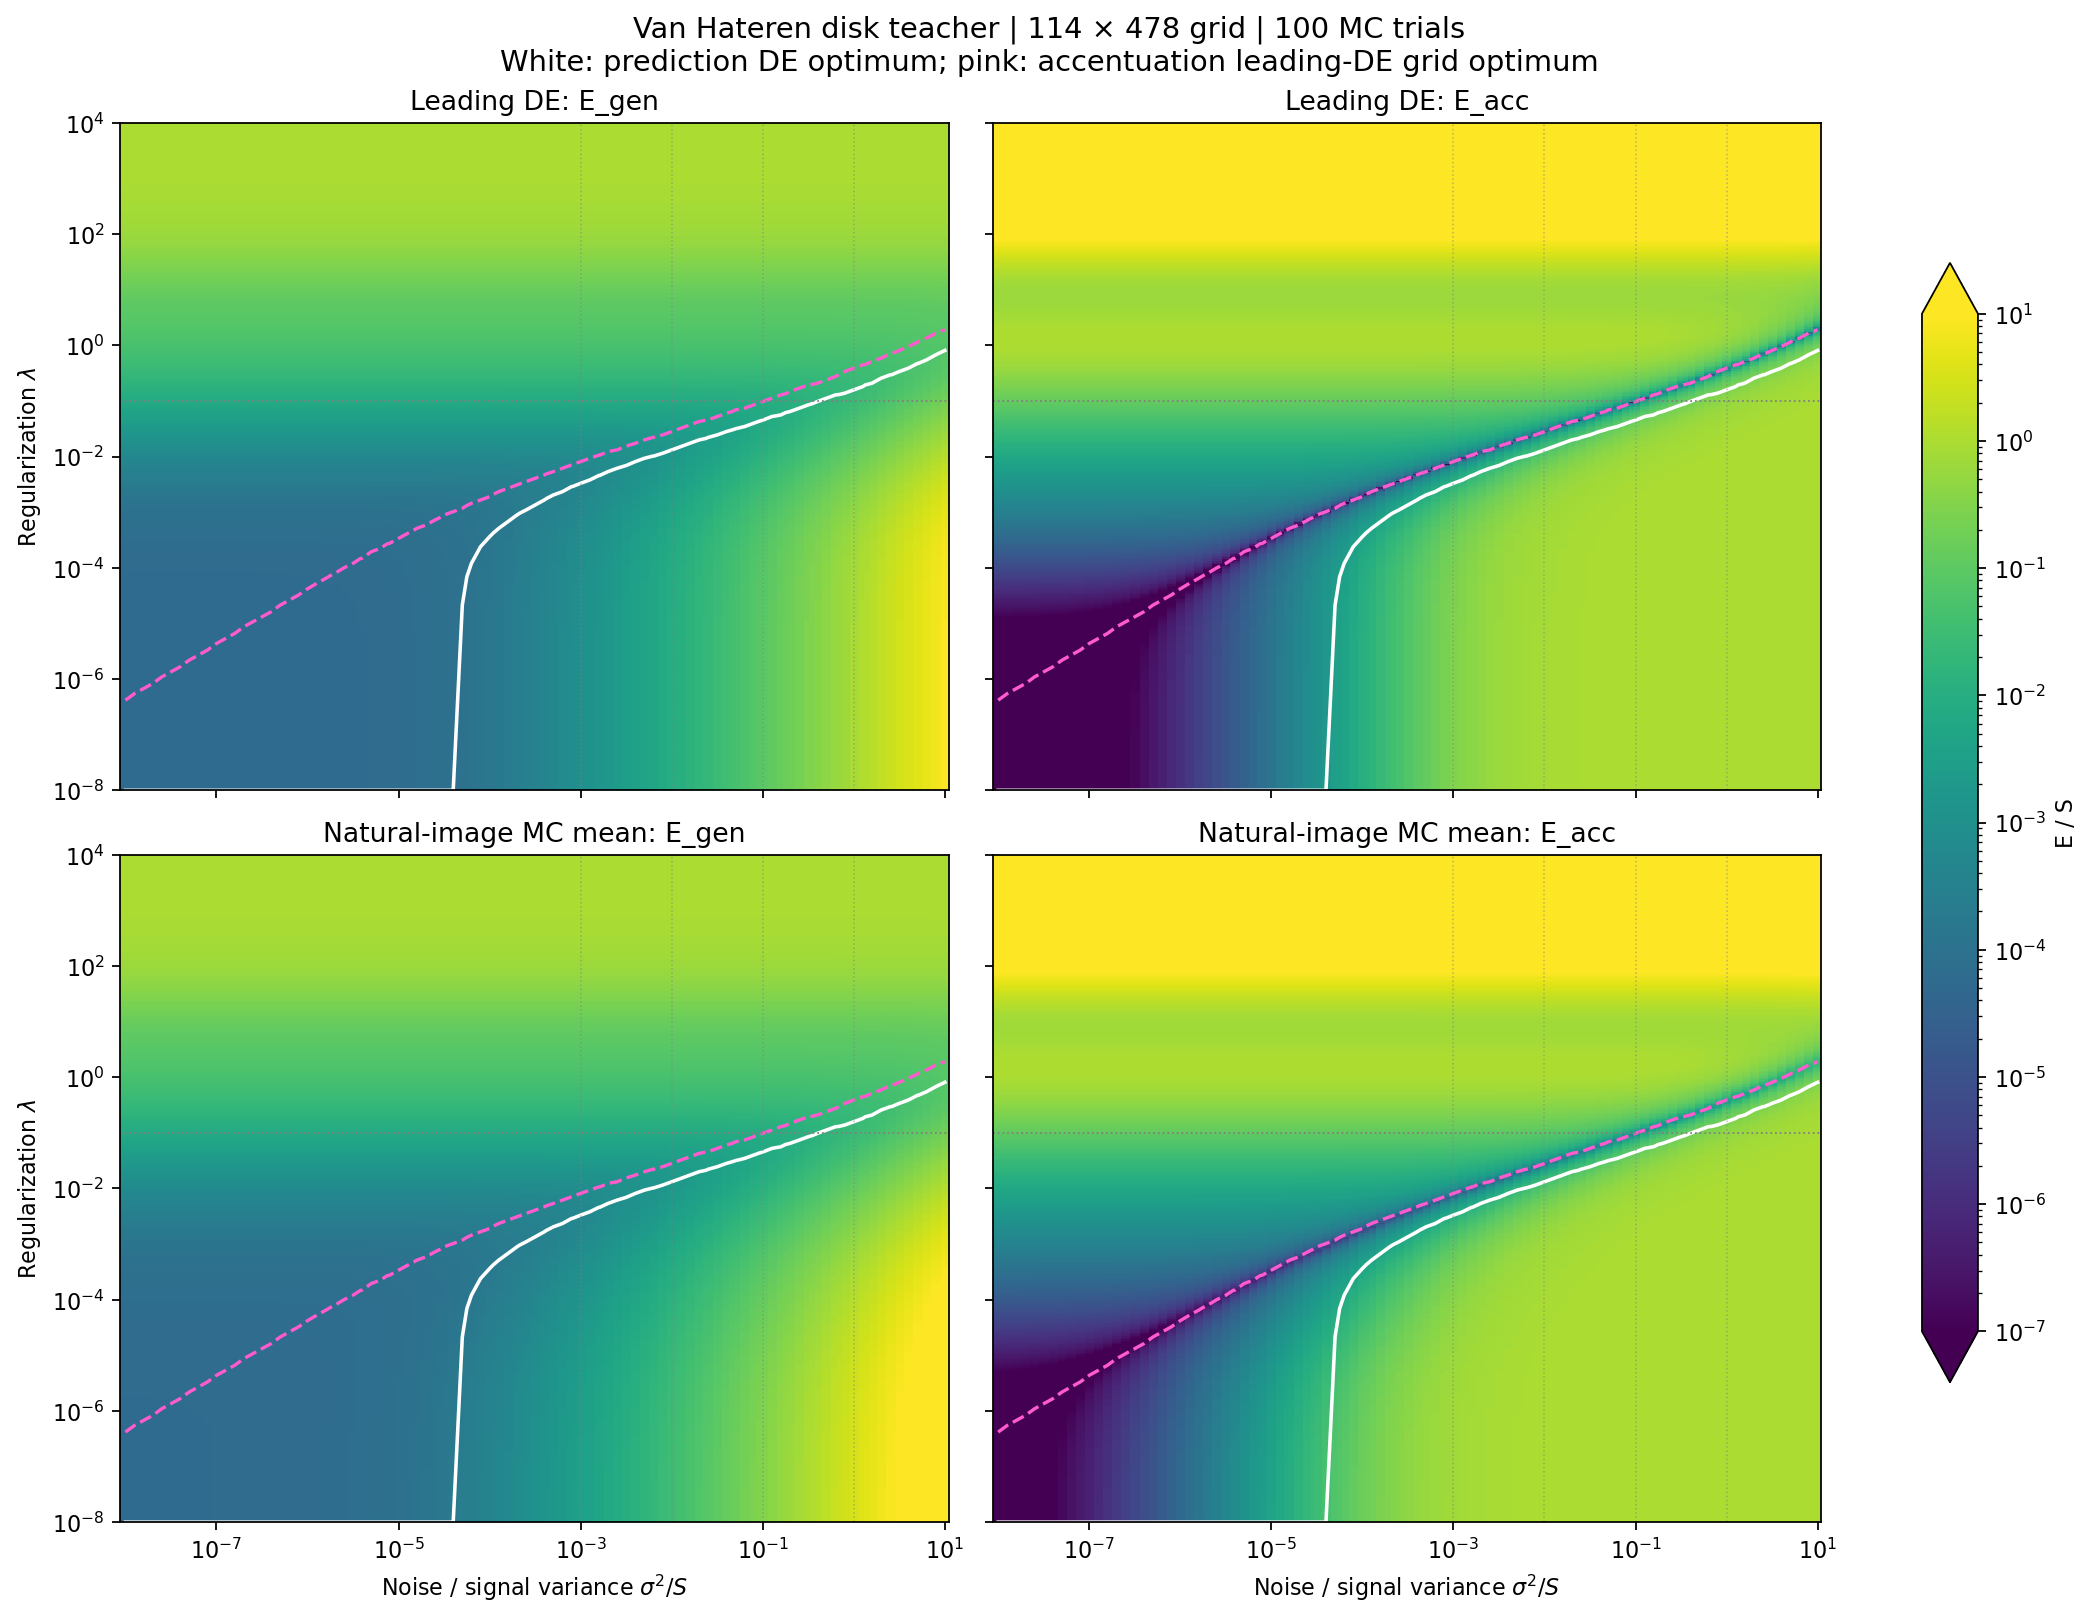
\includegraphics[width=0.48\linewidth,height=0.3\textheight,keepaspectratio]{figures/draft_landscape_error.png}\hfill
    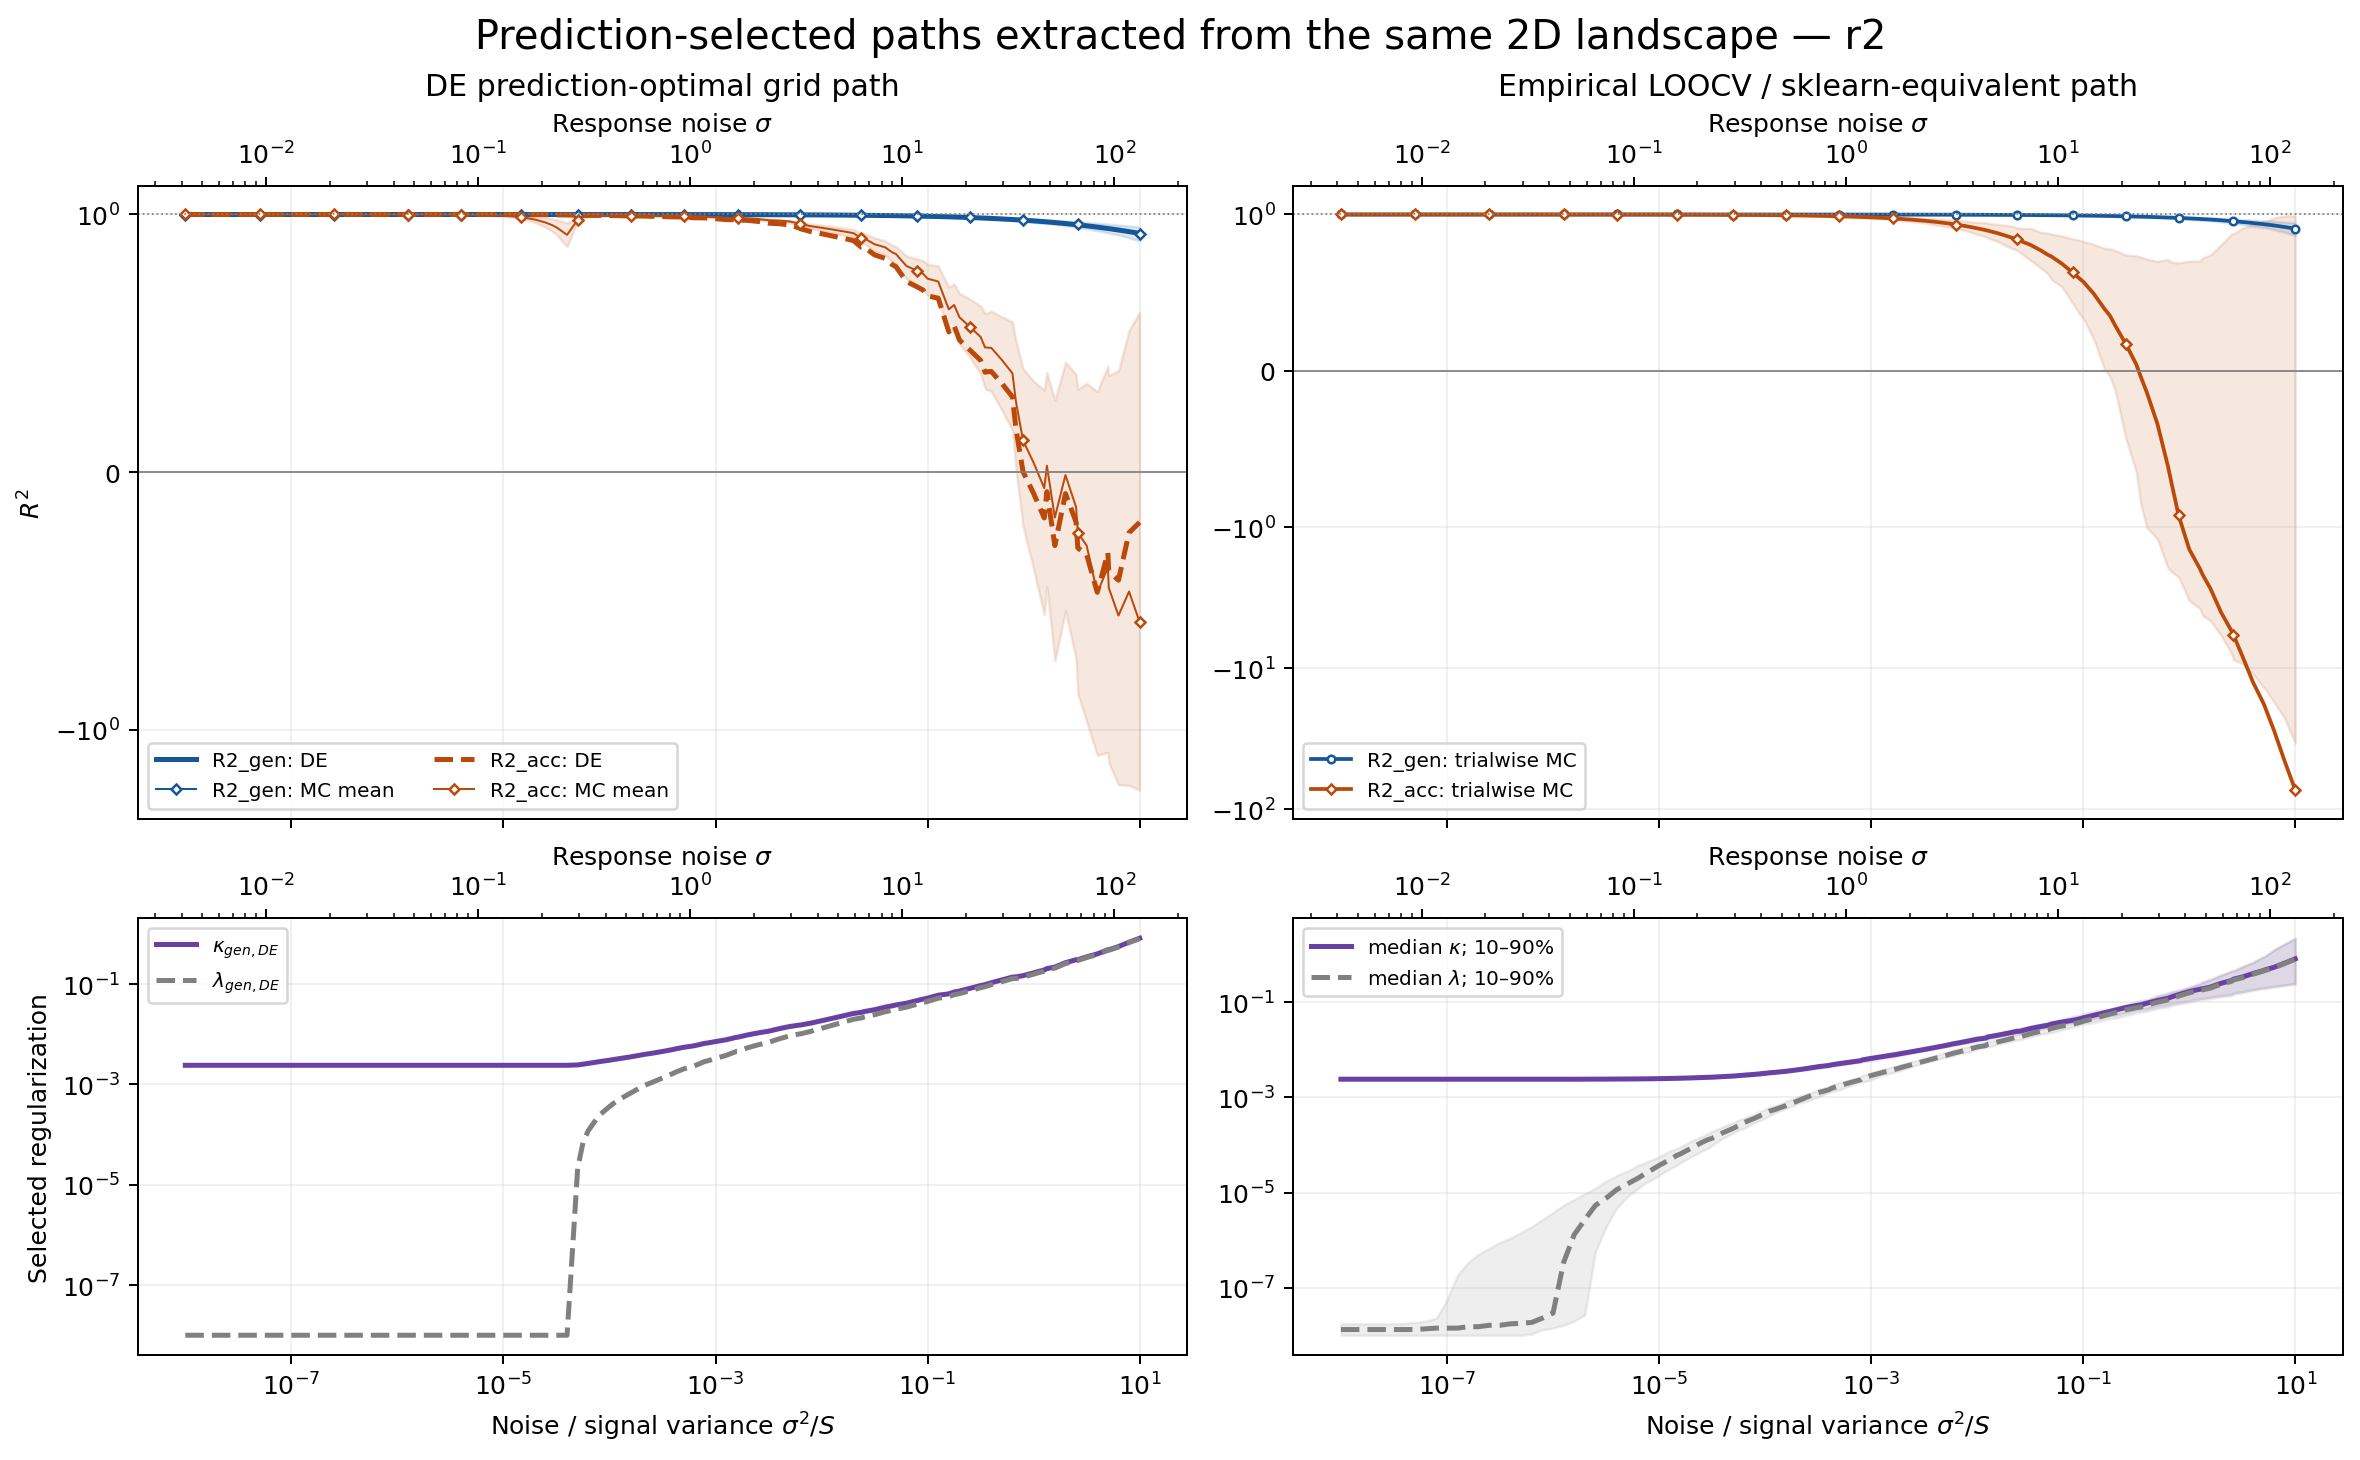
\includegraphics[width=0.5\linewidth,height=0.3\textheight,keepaspectratio]{figures/draft_slices_prediction_selected_r2.png}
    \caption{\textbf{Pixel ridge on van Hateren images ($d=10^4$, $n=10^3$, disk teacher).}
    \textbf{A}~Leading-DE control error $E_{acc}/S$ over noise $\sigma^2/S$ and penalty $\lambda$. The prediction-optimal path (white) and the control-calibrated path (pink) separate at all noise levels; Monte Carlo on real images (App.) reproduces the surface.
    \textbf{B}~Along the empirically cross-validated path, $R^2_{gen}$ stays above $0.9$ while $R^2_{acc}$ collapses once $\sigma^2/S\gtrsim0.1$; DE (lines) versus 100 natural-image trials (markers, 10--90\% band). Bottom: selected $\lambda$ and $\kappa$.}
    \label{fig:pixel}
\end{figure}

Figure~\ref{fig:pixel} confirms the picture on real natural-image regression. The DE surfaces track Monte Carlo over eight decades of noise; the prediction-optimal and control-calibrated penalties form two distinct ridges; and along the cross-validated path the student remains an excellent predictor while its accentuation $R^2$ becomes negative at moderate noise. 

\paragraph{Peer review: recognition without generation.}
Now evaluate $\bhat$ on the path of an independently fitted peer $\bprime$ at the same $\kappa$. The two noise realizations are uncorrelated, so the Euclidean noise term that inflates $D$ drops out of the cross products: ${\bhat}^\top\bprime\asymp B_{2,2}$ and ${\bstar}^\top\bprime\asymp B_{1,1}$, and the peer gain and score are
\begin{equation}
G_{peer}=\frac{{\bhat}^\top\bprime}{{\bstar}^\top\bprime}\asymp\frac{B_{2,2}}{B_{1,1}}\in(0,1],
\qquad
R^{2,(0)}_{peer}=1-\Big(1-\frac{B_{2,2}}{B_{1,1}}\Big)^2\in(0,1]
\label{eq:peer-de}
\end{equation}
(App.~\ref{prop:mr-peer}). Peer review measures only the shared shrinkage bias: at leading order it is never negative, degrades gracefully with noise, and is symmetric between the two fits. Self-evaluation instead carries the estimator's own Euclidean noise energy through Eq.~\ref{eq:pixel-de}, so $z_{acc}$ grows without bound with $\sigma^2/n$ and $R^2_{acc}$ becomes arbitrarily negative. A student can therefore track a peer's path while failing on its own, which is the linear form of Fig.~\ref{fig:phenomena}C. The asymmetry between a strong and a weak generator in the data arises when the two differ in noise energy, i.e. in their feature maps (Sec.~\ref{sec:feature}); and measured responses along a barely modulated path add trial noise that no evaluator can explain, which is why even the peer scores of a weak generator's images are poor.

\section{Feature-space ridge: the map decides what reaches the gradient}
\label{sec:feature}

Pixel regression explains why one student fails; it cannot explain why ten equally predictive backbones fail differently. We idealize a backbone as a fixed linear map $F\in\R^{p\times d}$, fit $\hat w$ by ridge on features $F\x$, and accentuate along the pixel gradient $\bhat=F^\top\hat w$. Let $C:=F\Sigma F^\top$ be the feature covariance and $G:=FF^\top$ the Euclidean feature Gram. The best realizable feature weight and its irreducible error are $w^\star=C^\dagger F\Sigma\bstar$ and $S_\perp=S-{w^\star}^\top Cw^\star$ (App.~\ref{lem:mr-feature-weights}).

\begin{prop}[Feature ridge: prediction and control]\label{prop:feature-de}\label{prop:linfeat_acc_ND}\label{prop:linfeat_gen_err}
With $\kappa$, $B^F$, $\mathrm{df}^F$ built from $(C,w^\star)$ and aspect ratio $p/n$,
\begin{equation}
E_{gen,DE}=\frac{n(\kappa^2B^F_{1,2}+S_\perp+\sigma^2)}{n-\mathrm{df}^F_2}-\sigma^2,\qquad
N_{DE}={\bstar}^\top\tilde\beta_\kappa,\qquad
D_{DE}=\|\tilde\beta_\kappa\|^2+\frac{E_{gen,DE}+\sigma^2}{n}\,T_F(\kappa),
\label{eq:feature-de}
\end{equation}
where $\tilde\beta_\kappa=F^\top(C+\kappa I)^{-1}F\Sigma\bstar$ is the mean pixel weight and
$T_F(\kappa):=\operatorname{Tr}[G(C+\kappa I)^{-2}C]$.
\end{prop}
Prediction sees the feature map only through $C$ and $F\Sigma\bstar$: the whole curve $E_{gen,DE}(\kappa)$, hence the cross-validated $\kappa$ and $R^2_{gen}$, is a function of $(C,F\Sigma\bstar,S,\sigma^2,n)$. Control additionally sees $G$, through $T_F$ and $\|\tilde\beta_\kappa\|$, and $F\bstar$, through $N_{DE}$ (Fig.~\ref{fig:feature}A). This is the statistical content of the dissociation: the prediction problem does not identify the control problem.

\begin{prop}[Prediction-preserving gauge]\label{prop:gauge}
For $\Sigma\succ0$ and any orthogonal $Q$ with $Q\Sigma^{1/2}\bstar=\Sigma^{1/2}\bstar$, the map $F\mapsto F\Sigma^{1/2}Q\Sigma^{-1/2}$ preserves $C$ and $F\Sigma\bstar$, hence the training law, $E_{gen,DE}(\kappa)$ and the DE cross-validated penalty, while changing $G$ and $F\bstar$ and therefore control.
\end{prop}
The gauge group is trivial for white data and grows with anisotropy. Rotating within it moves feature energy from high-variance to low-variance pixel directions at no cost to prediction (Fig.~\ref{fig:feature}B): along a continuous path, $E_{gen}$, $R^2_{gen}$ and the selected penalty are exactly constant, while $\operatorname{Tr}(FF^\top)$ grows by four orders of magnitude and $R^2_{acc}$ falls from near one to $-10^{8}$. Random draws from the family span this whole range (App.), so a population of equally predictive backbones with widely different control is the generic situation, not a construction.

\paragraph{What makes a map fragile.}
The factor $T_F$ is response-independent and has the spectral form (App.~\ref{prop:mr-fragility})
\begin{equation}
T_F(\kappa)=\sum_{k:s_k>0}\Big(\frac{s_k}{s_k+\kappa}\Big)^2\frac{\|g_k\|^2}{g_k^\top\Sigma g_k},
\qquad g_k:=F^\top v_k,
\label{eq:TF}
\end{equation}
with $(s_k,v_k)$ the eigenpairs of $C$. It averages, over the feature PCs that survive ridge shrinkage, the ratio between the Euclidean energy of the backpropagated PC gradient and its energy under the natural-image covariance. A map is fragile when its well-resolved feature directions backpropagate into low-variance, high-spatial-frequency pixel directions. This is the linear counterpart of the third observation of Sec.~\ref{sec:phenomena}, and it can be computed from the map and the image statistics alone.

\begin{center}
\fbox{\parbox{0.96\linewidth}{\small
\textbf{When is control fragile although prediction is fine?}
Holding the prediction error fixed, the leading control error (Eqs.~\ref{eq:pixel-de}, \ref{eq:pixel-zacc-cv}, \ref{eq:feature-de}) grows with three separable factors:
\textbf{(i) noise} $(E_{gen}+\sigma^2)/n$, the estimation-noise level, which is the only factor visible from held-out accuracy;
\textbf{(ii) spectrum} the mismatch between prediction-optimal and control-optimal penalties, Eq.~\ref{eq:pixel-zacc-cv}, which is zero for white data and grows with anisotropy and with teacher energy in low-variance modes;
\textbf{(iii) map} $T_F$, the ridge-weighted ratio of Euclidean to natural-covariance gradient energy, a property of the feature map alone.
Natural images make (ii) large for every model; the feature map decides (iii), and equally predictive maps can differ in it without bound.}}
\end{center}

\subsection{From the linear factor to a diagnostic for deep networks and neurons}
\label{sec:nonlinear}
For a nonlinear feature map $\phi$ with Jacobian $J_\phi(x)$ and natural-image feature covariance eigenpairs $(s_k,v_k)$, replacing $F$ by the local Jacobian in Eq.~\ref{eq:TF} gives
\begin{equation}
T_\phi(x,\kappa)=\sum_k\frac{s_k}{(s_k+\kappa)^2}\,\|J_\phi(x)^\top v_k\|^2,
\qquad
V_\phi:=\frac{E_{val}}{n}\,\E_x\big[T_\phi(x,\kappa)\big],
\label{eq:Tphi}
\end{equation}
where $J_\phi(x)^\top v_k=\nabla_x[v_k^\top\phi(x)]$ is the pixel gradient of feature PC $k$, obtainable by one backward pass per PC, and $V_\phi$ mirrors the variance term of Eq.~\ref{eq:feature-de}. For linear $\phi$ this is exact; for a network it is a diagnostic motivated by the theory, not a theorem, because the identity $s_k=g_k^\top\Sigma g_k$ that made $T_F$ a ratio of gradient energies no longer holds. Since an accentuation path travels far from the seed, we also evaluate smoothed versions in which the Jacobian is averaged, or the squared gradient is averaged, over a Gaussian neighborhood of the seed at pixel-noise scales from $0.5/255$ to $16/255$ (App.~\ref{sec:app-nonlinear-diagnostic}).

We computed these quantities for all 250 site--model pairs of the neuronal experiment, using each model's cross-validated ridge penalty and empirical feature spectrum to set $\kappa$, the ten experimental seed images for $\E_x$, and the held-out natural-image error of the control session for $E_{val}$. Because sites differ greatly in how controllable they are at all, we compare predictors after removing site means, so that each predictor is judged on ordering the ten models within a site (Fig.~\ref{fig:feature}C). Held-out prediction error carries essentially no information about which model will control better: its site-residual correlation with control slope is $0.03$ and with direct control error $-0.07$. The exact-local $V_\phi$ reaches $0.62$ with control slope and $0.44$ with control error across the nine trained models, and the trace $T_\phi$ alone does nearly as well, so the ordering comes from gradient geometry rather than from the prediction-error prefactor. Among the seven conventionally trained models the association is weaker but same-signed ($\approx0.2$ with slope), consistent with the two adversarially trained models being the strongest controllers and having by far the smallest $T_\phi$. Neighborhood-smoothed versions preserve or slightly improve the ordering. These are descriptive associations with repeated models within sites, not independent-sample tests, and they concern model ordering rather than absolute control error, for which the teacher-dependent terms of Eq.~\ref{eq:feature-de} would also be needed.

\begin{figure}[t]
    \centering
    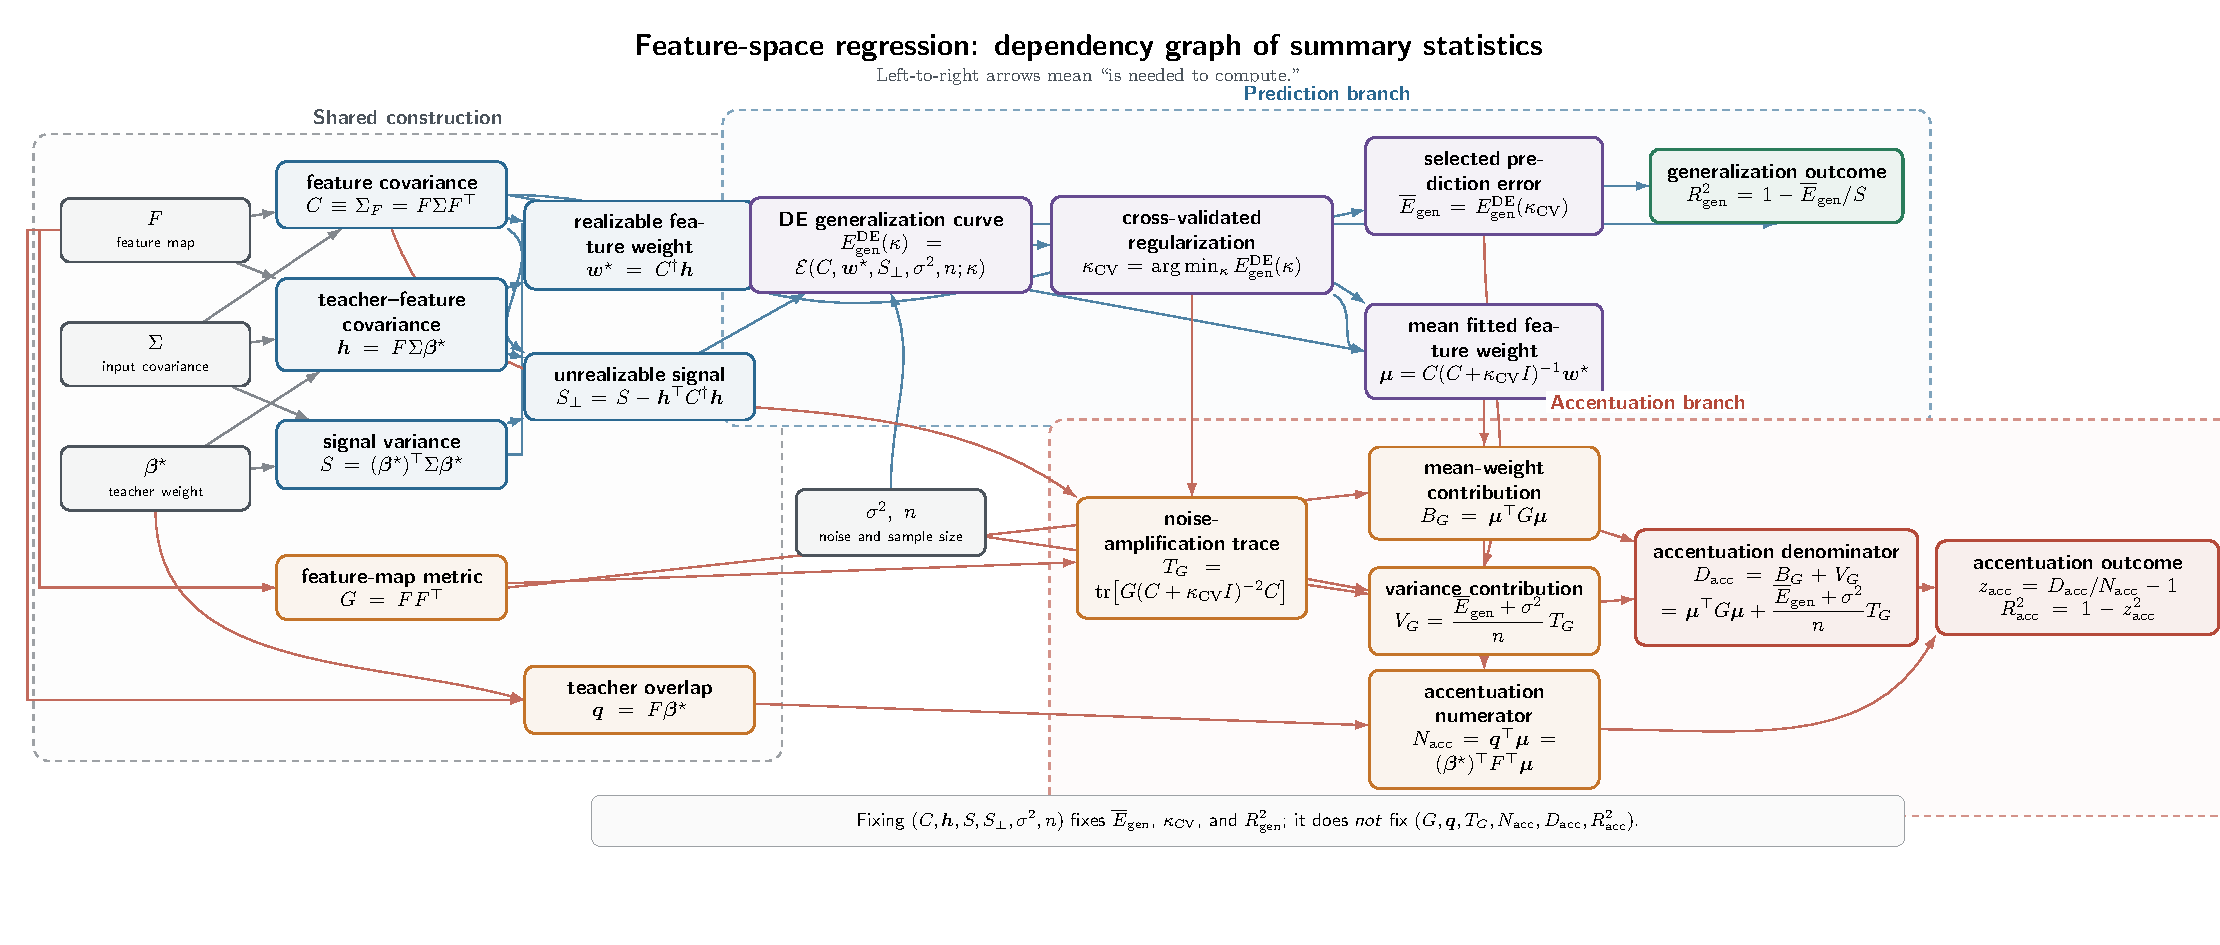
\includegraphics[width=0.55\linewidth,height=0.22\textheight,keepaspectratio]{figures/feature_summary_statistics_flow.pdf}\hfill
    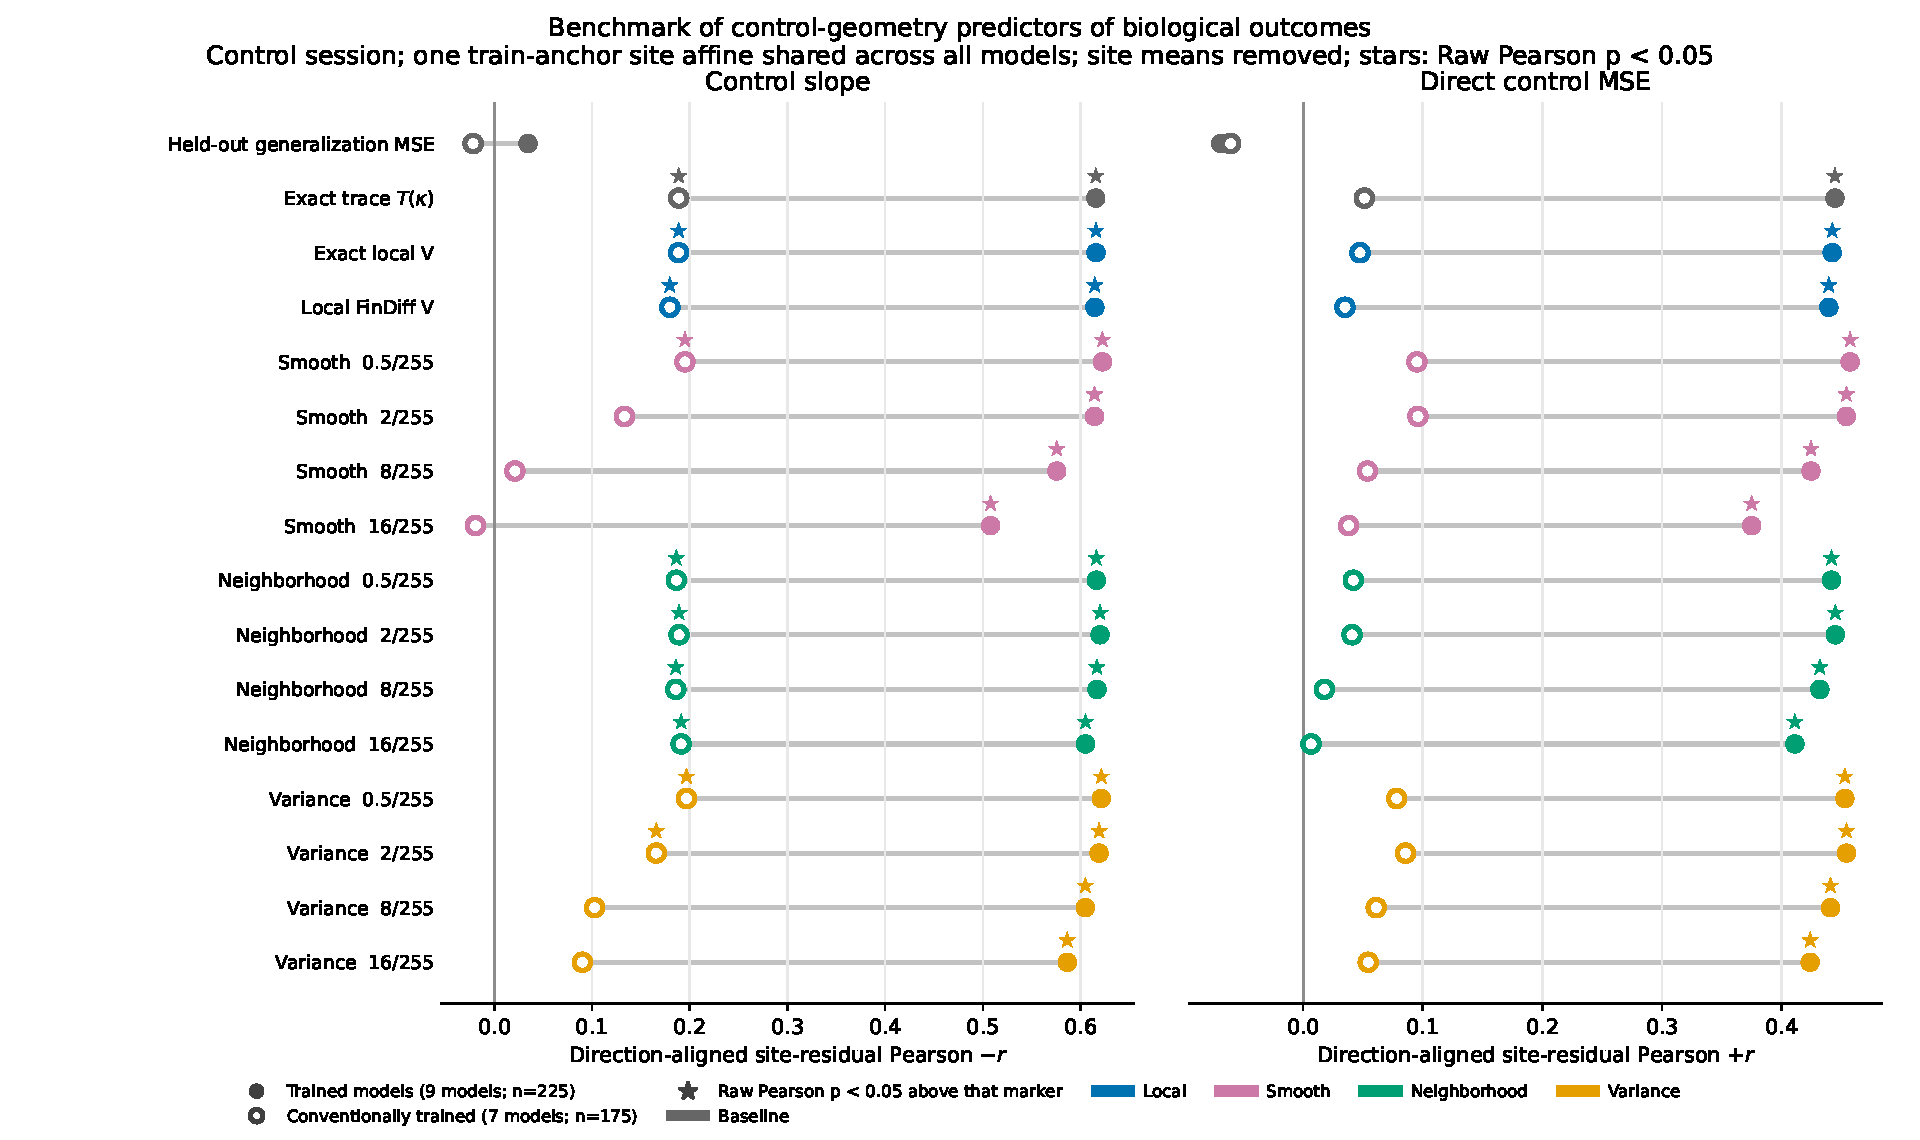
\includegraphics[width=0.44\linewidth,height=0.22\textheight,keepaspectratio]{figures/nonlinear_control_biological_validation.pdf}\\[2pt]
    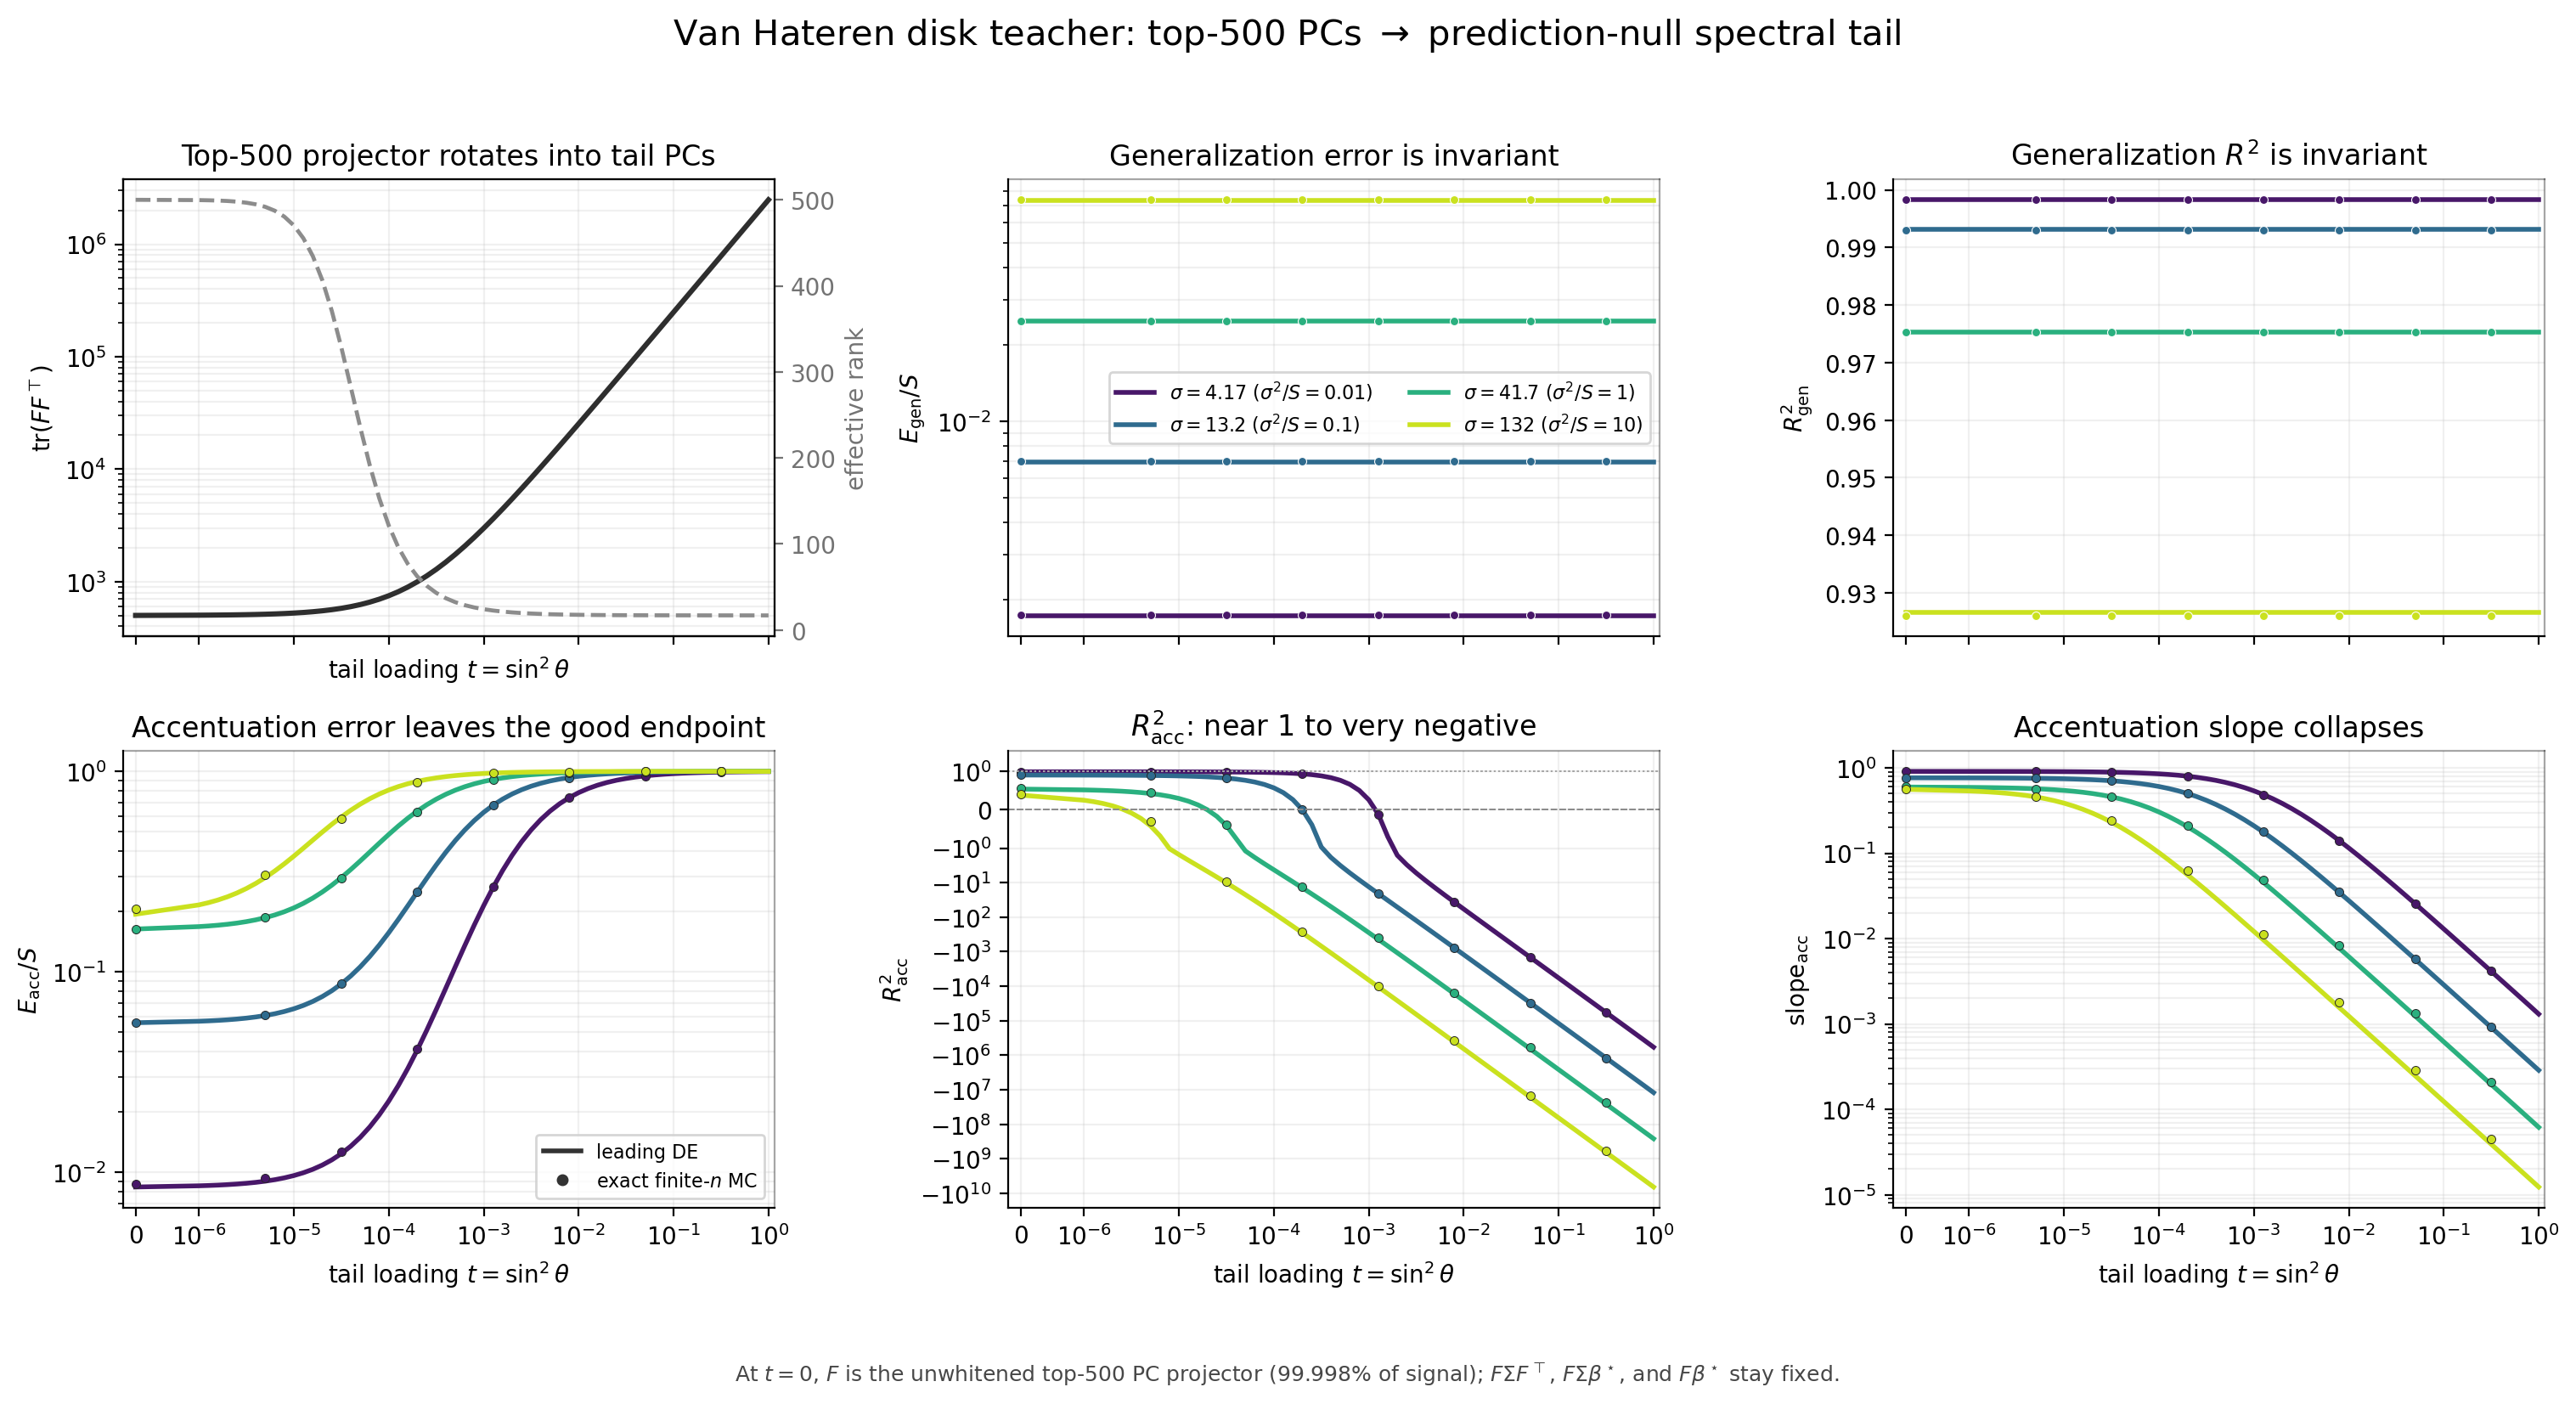
\includegraphics[width=\linewidth,height=0.2\textheight,keepaspectratio]{figures/VanHateren_Top500PC_prediction_null_feature_rotation.png}
    \caption{\textbf{Feature geometry decides control.}
    \textbf{A}~Dependency graph: $(C,F\Sigma\bstar,S,\sigma^2,n)$ fix generalization and the cross-validated penalty; control additionally needs $G=FF^\top$ and $F\bstar$ (draft: to be simplified to $\sim$8 boxes).
    \textbf{B}~Rotating a top-500-PC projector of van Hateren images into the prediction-null spectral tail: $E_{gen}$ and $R^2_{gen}$ are invariant while $R^2_{acc}$ and the slope collapse; DE (lines) matches finite-$n$ Monte Carlo (markers). (Draft: keep 3 of 6 panels.)
    \textbf{C}~Neuronal data: site-demeaned association of each candidate predictor with biological control slope (left) and control error (right) across nine trained (filled) and seven conventionally trained (open) models. Held-out error carries no model-order information; the exact trace, $V_\phi$ and its neighborhood versions do. (Draft: keep 5 rows.)}
    \label{fig:feature}\label{fig:nonlinear-biological-validation}
\end{figure}

\section{Discussion}
\label{sec:discussion}
A single mechanism accounts for the three neuronal phenomena: prediction measures weight error in the covariance metric, control measures it along the model's own gradient. In the linear theory the control error at fixed prediction error is governed by the three factors of the box in Sec.~\ref{sec:feature}: noise, spectrum, and map, of which only the first is visible from held-out accuracy. The practical implication is that selecting encoding models or penalties by held-out prediction cannot certify gradient-based control; validation must constrain the gradient, for instance through $T_\phi$, or test generated stimuli directly. The high-frequency artifacts of failed accentuations are not a cosmetic defect but the expected signature of low-variance directions that natural images never constrained.

\paragraph{Limitations.}
The theory assumes Gaussian inputs, a linear teacher, a fixed linear feature map and a one-dimensional accentuation path from a centered seed; the leading DEs predict typical fits and the location of the control optimum but not the fluctuation-dominated error at that optimum (App.~\ref{sec:app-ratio-corrections}). The nonlinear diagnostic is not a theorem, and its biological validation is descriptive. Extending the deterministic equivalents to learned nonlinear features and to curved accentuation trajectories is the natural next step.
